\section{Introduction}
In recent years, due to the progress of robot technology and the reduction in
cost, biomimetic robots have been increasingly used in animal behavior research.
Biomimetic robots are easier to operate than real animals, and their behavior
characteristics can be accurately controlled \cite{abdai_poking_the_futhre,
yeager_new_tech}. Through effective control methods and active guidance, these
robots can interact with animals, observe and record their reactions
\cite{son_entice_insect,Taylor2008frogs-17969,kopman_closed_loop_zebrafish,
partan_wild_tree,5650930}. Sometimes, biomimetic robots are placed in a group of
animals to explore their behavior mechanism, or to verify scientific assumptions
in the process of interaction \cite{doi:10.1126science.1144259,ward_quorum,
gribovskiy_mobile_robot,faria_novel_method}. For example, Kopman \textit{et al.}
studied the response of zebrafish to a robotic fish. The robotic fish is similar
to the real zebrafish in shape and color. The experimental results show that the
the response of zebrafish changes with the tail-beating pattern of the robotic
fish \cite{kopman_closed_loop_zebrafish}. Halloy \textit{et al.} introduced a
specially designed biomimetic autonomous robot into cockroaches to study the
collective decision-making behavior of cockroaches in shelter selection
\cite{doi:10.1126science.1144259}.

However, the mechanism
of state decision that ensures the two rats can interact with each other still
remains uncertain.

The social activities of rats have attracted the interest of many researchers,
and these studies have achieved remarkable results
\cite{fleliz_bidirectional_modulation,weiss_shall_two_walk}. Because of the
advantages of biomimetic robots in animal interactions, various rat-like robots
have been designed for the study of rats \cite{Lucas2018DesignOA,Shi_bb_2013,
Shi_bb_2015,shi-gao-tro-2022}. Ortiz \textit{et al.} designed a robotic rat
(e-puck) with a simple behavior pattern to explore whether the robot can
interact well with actual rats and trigger their social behaviors
\cite{Rusalky-sit}. Heath et al. developed a biomimetic robotic rat (Pirat),
which is similar in size to the real rat. The influence of the robot on rat
behaviors was tested by controlling different behaviors of the robot (frequent
approach and avoidance) \cite{pirat}. Sullivan \textit{et al.} designed a robot
imitating the behavior of rat pups, and planned the input/output cognitive
architecture for the robot through a genetic algorithm to deeply understand the
behavior of Norwegian rat pups \cite{sullivan-arl-2015}. However, these robots
have fewer degrees of freedom (DOFs) and lack flexibility in local motion, so it
is difficult to simulate the complex and diverse behavior patterns of rats. In
addition, the current research on robot-rat interaction usually adopts the
method of directly controlling the movement and behavior of the robot. The robot
acts as a stimulus to exert influence to observe the response of the target rat.
There are few studies on the behavioral interaction between rats. We believe
that learning the behavioral interaction of rats is indeed a means to promote
the effect of robot-rat interaction.

In this paper, we first constructed two behavior patterns of rat interaction:
the individual pattern and the interaction pattern. In our previous study, we
learned the individual behavior law of rats in the open field and applied it to
a small-scale robotic rat platform \cite{gao-eng-2022}. The robot has 4 DOFs in
the pitch direction and 3 DOFs in the yaw direction. It can perform movements
and behaviors similar to those of rats with a high degree of flexibility
\cite{shi-gao-tro-2021}. Therefore, we used the previously obtained behavior law
to build the individual pattern of rats.

Relatively, the interaction pattern of rats can be divided into different states,
such as tracking and imitating. The two rats participating in the interaction
process usually show different roles, one is the active stimulator and the other
is the passive receiver. The behavior of the receiver is determined by the
stimulator. When learning the behavioral interaction of rats, a difficult
problem is that the roles played by a rat usually change with each other. That
is, the same rat may be both a stimulator and a receiver at different times, and
it depends on the characteristics of the individual. Hence, we proposed the
following strategy: not distinguish the individual of rats, but only distinguish
the stimulator and receiver. The stimulator executes the individual pattern, and
the receiver switches between the individual pattern and the interaction
pattern. Which pattern the receiver executes depends on the probability of
interaction.

Furthermore, we learned the rat-like behavioral interaction by controlling the
interaction process of the two robots. The similarity of behavioral interaction
between robots and rats is measured by interaction information entropy. A
hypothesis concerning the behavioral interaction of rats is proposed; that is,
the probability of interaction between rats depends on the distance of the
centroid and the average relative velocity. According to the results of robot
interaction control and hypothesis test, we proved the rationality of the above
hypothesis, and obtained the optimal solution expressing their relationship.
Figure \ref{process-of-robot-learn} presents the process of robot learning
rat-like behavioral interaction. Robots learn similar behavior patterns and the
interaction process form rats to realize a more natural and effective robot-rat
interaction. This is of great significance to future robot-rat interactions.

\begin{figure}[h]
    \centering
    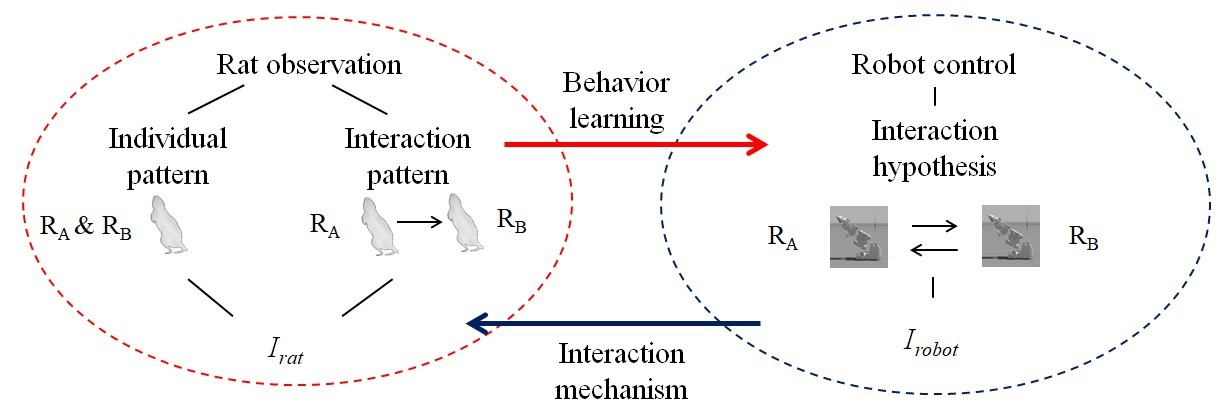
\includegraphics[width=0.8\textwidth]{process-of-robot-learn}
    \caption{The process of robot learning rat-like behavioral interaction.}
    \label{process-of-robot-learn}
\end{figure}

